\documentclass[aspectratio=169, table, 12pt]{beamer}

% Preamble bersama seluruh slide mata kuliah ini.
% Dipanggil dari slides/sessionXX/sessionXX.tex tepat sesudah baris
% \documentclass[aspectratio=169, table, 12pt]{beamer}
% Paket tambahan yang hanya dibutuhkan satu sesi ditulis di berkas sesi itu.

\usepackage{colortbl}
\usepackage{xcolor}
\usepackage{listings}
\usepackage{tabularx}
\usepackage{booktabs}
\usepackage{tikz}
\usepackage{pgfplots}
\pgfplotsset{compat=1.18}
\usetikzlibrary{arrows.meta, positioning, calc, fit, shapes.geometric,
	shapes.multipart, backgrounds, matrix, chains, trees}

\makeatletter
\def\input@path{{../theme/}}
\makeatother
\graphicspath{{../theme/}{../../figures/}}
\usetheme{Pradita}

\definecolor{praditagreen}{RGB}{37, 113, 71}

% Tema membuat garis tabel berwarna putih. Dikembalikan agar tabel terbaca.
\arrayrulecolor{black}
\setlength{\arrayrulewidth}{0.5pt}

\lstdefinelanguage{yaml}{
	basicstyle=\ttfamily\scriptsize,
	keywordstyle=\color{blue}\bfseries,
	commentstyle=\color{gray}\itshape,
	stringstyle=\color{red},
	showstringspaces=false,
	breaklines=true,
	frame=lines,
	numbers=none,
	backgroundcolor=\color{lightgray!10},
	tabsize=2,
	morecomment=[l]{\#}
}

\lstdefinelanguage{json}{
	basicstyle=\ttfamily\scriptsize,
	stringstyle=\color{red},
	commentstyle=\color{gray},
	breaklines=true,
	showstringspaces=false,
	tabsize=2,
	numbers=none,
	frame=lines,
	backgroundcolor=\color{lightgray!10},
	string=[s]{"}{"}
}

\lstdefinelanguage{bash}{
	keywords={},
	basicstyle=\ttfamily\scriptsize,
	ndkeywords={docker, kubectl, helm, curl, git, terraform},
	ndkeywordstyle=\color{purple}\bfseries,
	sensitive=true,
	commentstyle=\color{gray},
	numbers=none,
	breaklines=true,
	frame=lines,
	backgroundcolor=\color{lightgray!10},
	tabsize=2,
	comment=[l]{\#},
	showstringspaces=false
}

\lstdefinelanguage{http}{
	keywords={GET, POST, PUT, PATCH, DELETE, HEAD, OPTIONS, HTTP},
	basicstyle=\ttfamily\scriptsize,
	keywordstyle=\color{blue}\bfseries,
	sensitive=true,
	numbers=none,
	breaklines=true,
	frame=lines,
	backgroundcolor=\color{lightgray!10},
	tabsize=2,
	showstringspaces=false
}

\subtitle{IT40713 · Cloud-Native \& Microservices Architecture}
\author{\textbf{Alfa Yohannis}}


\title{\Huge Monolit hingga\\ \vspace{10pt} Microservices}

\begin{document}

\frame{\titlepage}

\begin{frame}
  \frametitle{Isi Pertemuan}
  \vspace{14pt}
  \begin{columns}[t]
    \column{0.5\textwidth}
    {\small\tableofcontents[sections={1-4}]}

    \column{0.5\textwidth}
    {\small\tableofcontents[sections={5-8}]}
  \end{columns}
\end{frame}

\begin{frame}{\hfill}
  \centering
  \Huge{\textbf{Bila \textit{microservices}\\sebagus itu, mengapa ada\\yang kembali ke monolit?}}
\end{frame}

\section{Tujuan dan Konteks}

\begin{frame}{\hfill}
  \centering
  \Huge{\textbf{Tujuan dan Konteks}}
\end{frame}

\begin{frame}{{\Large Tujuan Pembelajaran}}
  \vspace{10pt}
  \begin{itemize}
    \item Membandingkan monolit, \textit{modular monolith}, dan \textit{microservices} dari sisi
          manfaat dan biayanya.
    \item Mendiagnosis sumber keterkaitan (\textit{coupling}) pada aplikasi yang ada.
    \item Menuliskan keputusan gaya arsitektur dalam format ADR.
  \end{itemize}
\end{frame}

\begin{frame}{{\Large Tawaran Vendor kepada Medikara Health}}
  \vspace{10pt}
  \begin{itemize}
    \item Usulan: lima SIMRS diganti 32 layanan kecil dalam 18 bulan.
    \item Janji: rilis mandiri, skala mandiri, banyak tim bekerja sekaligus.
    \item Pertanyaan direktur keuangan: mengapa ada perusahaan yang kembali ke monolit?
    \item \textit{Microservices} adalah gaya arsitektur, bukan tujuan.
    \item Ada titik tengah yang sering terlewat: \textit{modular monolith}.
  \end{itemize}
\end{frame}

\begin{frame}{{\Large Diagram Konsep Bab 7}}
  \centering
  {\small\bfseries Batas modul dipilih sebelum distribusi layanan}\par\medskip
  \adjustbox{width=0.96\textwidth,height=0.7\textheight,keepaspectratio}{%
    % Diagram konsep Bab 7: Batas modul dipilih sebelum distribusi layanan.
% Dibangkitkan tools/render-diagrams.py dari figures/chapter-diagrams.json;
% ubah data JSON lalu jalankan ulang skrip, jangan sunting berkas ini langsung.
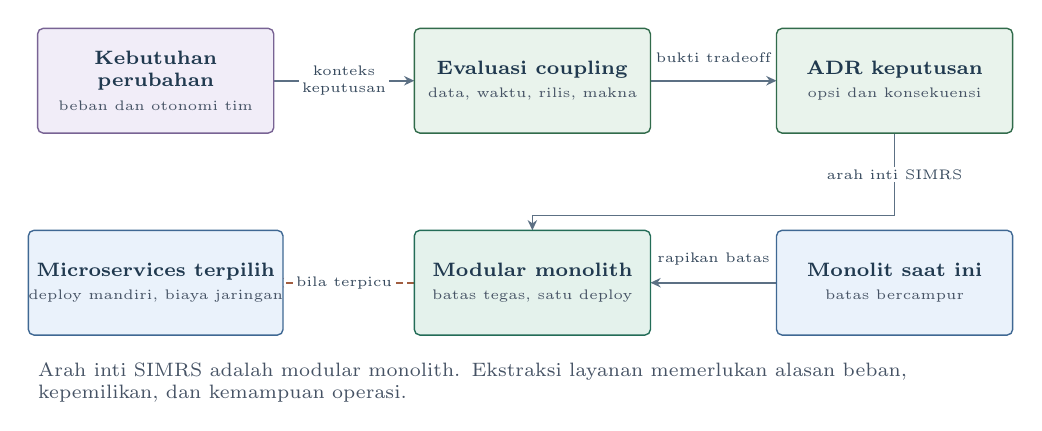
\begin{tikzpicture}[
  x=0.92cm, y=0.95cm,
  kotak konsep/.style={draw, line width=0.5pt, rounded corners=2pt,
    align=center, minimum width=2.999cm,
    minimum height=1.330cm, inner sep=0pt, font=\scriptsize,
    text=konsepJudul},
  peran actor/.style={kotak konsep, fill=konsepIsiActor, draw=konsepGarisActor},
  peran service/.style={kotak konsep, fill=konsepIsiService, draw=konsepGarisService},
  peran control/.style={kotak konsep, fill=konsepIsiControl, draw=konsepGarisControl},
  peran data/.style={kotak konsep, fill=konsepIsiData, draw=konsepGarisData},
  peran outcome/.style={kotak konsep, fill=konsepIsiOutcome, draw=konsepGarisOutcome},
  peran risk/.style={kotak konsep, fill=konsepIsiRisk, draw=konsepGarisRisk},
  panah konsep/.style={-{Stealth[length=1.3mm, width=1.2mm]}, line width=0.6pt,
    draw=konsepPanah},
  panah putus/.style={panah konsep, draw=konsepPanahPutus,
    dash pattern=on 2.5pt off 1.5pt},
  label panah/.style={font=\tiny, align=center, fill=white,
    inner sep=1pt, text=konsepLabel},
  catatan/.style={font=\scriptsize, align=left, anchor=north west,
    inner sep=0pt, text width=12.383cm, text=konsepTeks,
    execute at begin node={\hyphenpenalty=10000\hbadness=10000\relax}},
]
  \definecolor{konsepIsiActor}{HTML}{EEF1F6}
  \definecolor{konsepGarisActor}{HTML}{50627D}
  \definecolor{konsepIsiService}{HTML}{EAF2FB}
  \definecolor{konsepGarisService}{HTML}{3F6893}
  \definecolor{konsepIsiControl}{HTML}{E9F3EC}
  \definecolor{konsepGarisControl}{HTML}{316B4B}
  \definecolor{konsepIsiData}{HTML}{F1EDF8}
  \definecolor{konsepGarisData}{HTML}{786394}
  \definecolor{konsepIsiOutcome}{HTML}{E4F2EC}
  \definecolor{konsepGarisOutcome}{HTML}{236C57}
  \definecolor{konsepIsiRisk}{HTML}{FCEDE7}
  \definecolor{konsepGarisRisk}{HTML}{B36947}
  \definecolor{konsepJudul}{HTML}{20394F}
  \definecolor{konsepTeks}{HTML}{455264}
  \definecolor{konsepLabel}{HTML}{35485C}
  \definecolor{konsepPanah}{HTML}{5C7084}
  \definecolor{konsepPanahPutus}{HTML}{A15D40}
  % Panah dan label lebih dahulu; kotak menutupi sisa latar label.
  \draw[panah konsep] (0.93,0) -- (2.87,0);
  \draw[panah konsep] (6.13,0) -- (7.87,0);
  \draw[panah konsep] (7.87,-2.7) -- (6.13,-2.7);
  \draw[panah konsep] (9.5,-0.7) -- (9.5,-1.8) -- (4.5,-1.8) -- (4.5,-2);
  \draw[panah putus] (2.87,-2.7) -- (0.93,-2.7);
  \node[label panah] at (1.9,0) {konteks\\keputusan};
  \node[label panah] at (7,0.31) {bukti tradeoff};
  \node[label panah] at (7,-2.39) {rapikan batas};
  \node[label panah] at (9.5,-1.25) {arah inti SIMRS};
  \node[label panah] at (1.9,-2.7) {bila terpicu};
  \node[peran data] (kebutuhan) at (-0.7,0)
    {\textbf{Kebutuhan}\\\textbf{perubahan}\\[0.5pt]{\tiny\color{konsepTeks}beban dan otonomi tim}};
  \node[peran control] (coupling) at (4.5,0)
    {\textbf{Evaluasi coupling}\\[0.5pt]{\tiny\color{konsepTeks}data, waktu, rilis, makna}};
  \node[peran control] (adr) at (9.5,0)
    {\textbf{ADR keputusan}\\[0.5pt]{\tiny\color{konsepTeks}opsi dan konsekuensi}};
  \node[peran service] (micro) at (-0.7,-2.7)
    {\textbf{Microservices terpilih}\\[0.5pt]{\tiny\color{konsepTeks}deploy mandiri, biaya jaringan}};
  \node[peran outcome] (modul) at (4.5,-2.7)
    {\textbf{Modular monolith}\\[0.5pt]{\tiny\color{konsepTeks}batas tegas, satu deploy}};
  \node[peran service] (mono) at (9.5,-2.7)
    {\textbf{Monolit saat ini}\\[0.5pt]{\tiny\color{konsepTeks}batas bercampur}};
  \node[catatan] at (-2.33,-3.77)
    {Arah inti SIMRS adalah modular monolith. Ekstraksi layanan memerlukan alasan beban, kepemilikan, dan kemampuan operasi.};
\end{tikzpicture}
}
\end{frame}

\section{Tiga Gaya Arsitektur}

\begin{frame}{\hfill}
  \centering
  \Huge{\textbf{Tiga Gaya Arsitektur}}
\end{frame}

\begin{frame}{{\Large Monolit}}
  \vspace{10pt}
  \begin{itemize}
    \item Seluruh fungsi dibangun, diuji, dan dirilis sebagai satu unit.
    \item Umumnya satu proses dan satu basis data bersama.
    \item Paling sederhana untuk tim kecil dan domain yang belum stabil.
    \item Masalah muncul bila tumbuh tanpa batas internal yang dijaga.
  \end{itemize}
  \vspace{6pt}
  {\small Analogi: rumah makan dengan satu dapur. Cocok saat kecil, sesak saat seratus kursi.}
\end{frame}

\begin{frame}{{\Large Modular Monolith}}
  \vspace{10pt}
  \begin{itemize}
    \item Tetap satu unit rilis.
    \item Dibagi menjadi modul dengan batas tegas dan antarmuka publik.
    \item Data setiap modul dipisah, misalnya skema basis data sendiri.
    \item Batas dijaga aturan tertulis dan alat pemeriksa otomatis.
  \end{itemize}
  \vspace{6pt}
  {\small Analogi: rumah sakit satu kompleks bersayap. Laboratorium meminta reagen lewat loket
  farmasi, bukan masuk ke gudangnya.}
\end{frame}

\begin{frame}{{\Large Microservices}}
  \vspace{10pt}
  \begin{itemize}
    \item Lewis dan Fowler: sekumpulan layanan kecil, masing-masing dalam prosesnya sendiri.
    \item Berkomunikasi lewat mekanisme ringan, mengikuti kapabilitas bisnis.
    \item Newman: layanan yang dapat dirilis mandiri, dimodelkan di sekitar domain.
    \item Kata kuncinya dirilis mandiri; ukuran kecil bukan tujuan.
  \end{itemize}
  \vspace{6pt}
  {\small Analogi: permukiman rumah kecil. Renovasi mandiri, tetapi barang harus lewat jalan
  yang bisa macet.}
\end{frame}

\begin{frame}{{\Large Spektrum, Bukan Pilihan Biner}}
  \centering
  \eadiagram{../../figures/ch07-spektrum-gaya.tex}
\end{frame}

\begin{frame}{{\Large Perbandingan Tiga Gaya}}
  \footnotesize
  \begin{tabularx}{\textwidth}{>{\raggedright\arraybackslash}p{2.8cm}
      >{\raggedright\arraybackslash}X >{\raggedright\arraybackslash}X
      >{\raggedright\arraybackslash}X}
    \hline
    \textbf{Aspek} & \textbf{Monolit} & \textbf{\textit{Modular monolith}} &
      \textbf{\textit{Microservices}} \\
    \hline
    Unit rilis & Satu & Satu & Satu per layanan \\
    \hline
    Batas antarbagian & Longgar & Tegas, dijaga alat & Tegas, dipisah jaringan \\
    \hline
    Data & Satu basis data bersama & Skema per modul & Basis data per layanan \\
    \hline
    Penskalaan & Seluruh sistem & Seluruh sistem & Per layanan \\
    \hline
    Syarat tim dan otomasi & Rendah & Sedang & Tinggi \\
    \hline
    Cocok untuk & Tim kecil, domain belum jelas & Beberapa tim, satu jadwal rilis & Banyak
      tim yang perlu rilis mandiri \\
    \hline
  \end{tabularx}

  \vspace{8pt}
  \small Jebakan: monolit terdistribusi, dipisah jaringan tetapi tetap dirilis bersama.
\end{frame}

\begin{frame}{{\Large Contoh Nyata dan Titik Awal Medikara}}
  \vspace{10pt}
  \begin{itemize}
    \item Shopify: lebih dari seribu pengembang, lebih dari sepuluh tahun; memilih
          \textit{modular monolith}.
    \item Sekitar 6.000 kelas program dipetakan ke komponen seperti pesanan dan penagihan.
    \item Medikara: lima SIMRS, versi 3.9 (Bandung) sampai 5.2 (Jakarta).
    \item Setiap salinan monolit dengan sembilan modul dan satu basis data.
    \item Pertanyaan yang tepat: satu sistem atau lima, dengan batas atau tanpa batas?
  \end{itemize}
\end{frame}

\section{Coupling dan Biaya Terdistribusi}

\begin{frame}{\hfill}
  \centering
  \Huge{\textbf{Coupling dan Biaya\\Sistem Terdistribusi}}
\end{frame}

\begin{frame}{{\Large Coupling dan Cohesion}}
  \vspace{10pt}
  \begin{itemize}
    \item \textit{Coupling}: derajat ketergantungan antarbagian.
    \item \textit{Cohesion}: derajat keterkaitan isi di dalam satu bagian.
    \item Arah yang dicari: \textit{coupling} rendah, \textit{cohesion} tinggi.
    \item \textit{Coupling} tampak (di diagram) dan tersembunyi (di riwayat perubahan).
  \end{itemize}
  \vspace{6pt}
  {\small Analogi: panitia pernikahan. Seksi konsumsi mengganti menu tanpa rapat dengan seksi
  dekorasi.}
\end{frame}

\begin{frame}{{\Large Empat Jenis Coupling}}
  \footnotesize
  \begin{tabularx}{\textwidth}{>{\raggedright\arraybackslash}p{1.6cm}
      >{\raggedright\arraybackslash}X >{\raggedright\arraybackslash}X}
    \hline
    \textbf{Jenis} & \textbf{Tanda di lapangan} & \textbf{Contoh di Medikara} \\
    \hline
    Data & Satu perubahan kolom memaksa banyak bagian diuji ulang & Aplikasi apotek membaca
      tabel SIMRS langsung \\
    \hline
    Waktu & Gangguan satu sistem menghentikan sistem lain & Janji temu Medikara+ berhenti saat
      SIMRS dipelihara \\
    \hline
    Rilis & Jadwal rilis menunggu tim lain & Perubahan tarif menunggu rilis modul klaim \\
    \hline
    Makna & Arti satu kode berubah, bagian lain salah tafsir & Status ``pulang'' berbeda arti di
      rawat inap dan penagihan \\
    \hline
  \end{tabularx}
\end{frame}

\begin{frame}{{\Large Coupling Data pada SIMRS}}
  \centering
  \eadiagram{../../figures/ch07-coupling-data.tex}
\end{frame}

\begin{frame}{{\Large Fallacies of Distributed Computing}}
  \footnotesize
  \begin{tabularx}{\textwidth}{>{\raggedright\arraybackslash}p{4.2cm}
      >{\raggedright\arraybackslash}X}
    \hline
    \textbf{Asumsi keliru} & \textbf{Akibat bagi organisasi} \\
    \hline
    Jaringan selalu andal & Setiap panggilan perlu pengulangan dan penanganan gagal \\
    \hline
    Latensi nol & Permintaan lewat banyak layanan terasa lambat \\
    \hline
    \textit{Bandwidth} tidak terbatas & Citra radiologi membebani jaringan \\
    \hline
    Jaringan aman & Otentikasi dan enkripsi di setiap layanan \\
    \hline
    Topologi tidak berubah & Alamat layanan dicari secara dinamis \\
    \hline
    Hanya ada satu administrator & Koordinasi lintas tim dan kontrak \\
    \hline
    Biaya transpor nol & Tagihan transfer data dan pemantauan naik \\
    \hline
    Jaringan seragam & Pengujian banyak kombinasi lingkungan \\
    \hline
  \end{tabularx}
\end{frame}

\begin{frame}{{\Large Biaya Jaringan Dapat Dihitung}}
  \vspace{10pt}
  \begin{itemize}
    \item Pemesanan janji temu melewati enam layanan berurutan.
    \item Setiap layanan tersedia 99,9 persen.
    \item Rangkaian: $0{,}999^{6} \approx 0{,}994$, sekitar 99,4 persen.
    \item Sebulan 30 hari: satu layanan boleh mati sekitar 43 menit.
    \item Rangkaian enam layanan: sekitar 4 jam 19 menit.
  \end{itemize}
  \vspace{6pt}
  {\small Biaya lain: data (Bab 10), pengujian, dan operasi (Bab 11 dan 13).}
\end{frame}

\begin{frame}{{\Large Kasus Medikara: Diagnosis SIMRS Jakarta}}
  \footnotesize
  \begin{tabularx}{\textwidth}{>{\raggedright\arraybackslash}p{2.4cm} r r
      >{\raggedright\arraybackslash}X}
    \hline
    \textbf{Modul} & \textbf{Perubahan} & \textbf{Gangguan} & \textbf{Pasangan paling erat} \\
    \hline
    Pendaftaran & 9 & 9 & Rekam medis (5) \\
    \hline
    Rekam medis & 13 & 6 & Pendaftaran (5) \\
    \hline
    Laboratorium & 5 & 4 & Rekam medis (4) \\
    \hline
    Penagihan & 17 & 11 & Klaim BPJS (10) \\
    \hline
    Klaim BPJS & 13 & 22 & Penagihan (10) \\
    \hline
    Empat modul lain & 19 & 11 & Tidak ada yang menonjol \\
    \hline
    \textbf{Jumlah} & \textbf{76} & \textbf{63} & Dari 40 permintaan; 30 (75 persen) lintas
      modul \\
    \hline
  \end{tabularx}

  \vspace{6pt}
  \small Klaim dan penagihan: derajat 67 persen, kandidat satu modul dan satu tim.
\end{frame}

\section{Hukum Conway}

\begin{frame}{\hfill}
  \centering
  \Huge{\textbf{Hukum Conway\\dan Struktur Tim}}
\end{frame}

\begin{frame}{{\Large Struktur Komunikasi Membentuk Sistem}}
  \vspace{10pt}
  \begin{itemize}
    \item Conway (1968): rancangan sistem meniru struktur komunikasi organisasinya.
    \item Tim yang jarang berbicara menghasilkan bagian terpisah yang kaku.
    \item Bukti empiris: organisasi yang longgar cenderung menghasilkan produk lebih modular.
  \end{itemize}
  \vspace{6pt}
  {\small Analogi: satu RW dengan lima RT yang masing-masing mengatur keamanan sendiri. Tamu
  ditanyai berkali-kali.}
\end{frame}

\begin{frame}{{\Large Manuver Conway Terbalik}}
  \vspace{10pt}
  \begin{itemize}
    \item Tim ditata lebih dahulu sesuai arsitektur yang diinginkan.
    \item Tim stabil, kecil, sekitar lima sampai sembilan orang.
    \item Tanggung jawab dibatasi beban kognitif tim.
    \item \textit{Microservices} butuh satu tim pemilik per layanan.
    \item Team Topologies dibahas rinci di Bab 13.
  \end{itemize}
\end{frame}

\begin{frame}{{\Large Hukum Conway pada SIMRS}}
  \centering
  \eadiagram{../../figures/ch07-hukum-conway.tex}
\end{frame}

\begin{frame}{{\Large Kasus Medikara: Tim TI per Rumah Sakit}}
  \vspace{10pt}
  \begin{itemize}
    \item 26 orang TI di lima rumah sakit; 12 orang mengubah kode SIMRS.
    \item Lima struktur komunikasi menghasilkan lima SIMRS.
    \item Usulan: empat tim domain, tiga pengembang dan dua orang unit pengguna per tim.
    \item Konsekuensi organisasi: direktur rumah sakit tidak lagi punya tim pengembang.
    \item Konsekuensi teknis: 32 layanan berarti delapan layanan per tim.
  \end{itemize}
\end{frame}

\section{Kapan Microservices Tidak Tepat}

\begin{frame}{\hfill}
  \centering
  \Huge{\textbf{Kapan Microservices\\Tidak Tepat}}
\end{frame}

\begin{frame}{{\Large Lima Tanda Belum Siap}}
  \footnotesize
  \begin{tabularx}{\textwidth}{>{\raggedright\arraybackslash}p{4.0cm}
      >{\raggedright\arraybackslash}X}
    \hline
    \textbf{Tanda} & \textbf{Pertanyaan pemeriksa} \\
    \hline
    Batas domain belum stabil & Sudahkah \textit{bounded context} diuji dengan data perubahan? \\
    \hline
    Layanan melebihi kemampuan tim & Berapa layanan yang dipegang setiap tim? \\
    \hline
    Rilis masih manual & Berapa langkah manual dalam satu rilis? \\
    \hline
    Pemantauan belum terpusat & Dapatkah satu permintaan ditelusuri lintas sistem? \\
    \hline
    Tidak ada alasan bisnis terukur & Masalah apa yang hanya selesai dengan rilis dan skala
      mandiri? \\
    \hline
  \end{tabularx}
\end{frame}

\begin{frame}{{\Large Pelajaran dari Segment (Noonan, 2018)}}
  \vspace{10pt}
  \begin{itemize}
    \item Satu layanan per tujuan pengiriman: lebih dari 140 layanan.
    \item Versi pustaka bersama menyimpang; tiga insinyur sibuk menjaga sistem.
    \item Disatukan menjadi satu layanan; pengujian dari sampai satu jam ke milidetik.
    \item Perbaikan pustaka bersama: 32 per tahun, lalu 46 setahun setelah monolit.
    \item Harganya: satu kesalahan dapat menghentikan semua tujuan.
  \end{itemize}
\end{frame}

\begin{frame}{{\Large Monolith First dan Pendapat Sebaliknya}}
  \vspace{10pt}
  \begin{itemize}
    \item Fowler: kisah sukses umumnya berawal dari monolit yang kemudian dipecah.
    \item Tilkov: sistem baru adalah saat terbaik memisahkan bagian, bila domain dipahami.
    \item Titik temu: pemahaman domain menentukan.
    \item Medikara: batas \textit{bounded context} baru dipetakan, belum diuji.
    \item Jalan tengah: uji batas di \textit{modular monolith}, pecah bila data membuktikan.
  \end{itemize}
\end{frame}

\begin{frame}{{\Large Kasus Medikara: Menimbang Usulan 32 Layanan}}
  \vspace{10pt}
  \begin{itemize}
    \item Batas domain baru dipetakan di Bab 6, belum diuji.
    \item 12 pengembang dan 6 orang tim platform: $32/18 \approx 1{,}8$ layanan per orang.
    \item Rilis Medikara+ masih 37 langkah manual; pemantauan masih per sistem.
    \item Alasan bisnis terukur hanya satu: lonjakan janji temu sekitar 60 persen.
    \item Calon pertama untuk dipisah: pemesanan janji temu, setelah otomasi siap.
  \end{itemize}
\end{frame}

\section{Architecture Decision Record}

\begin{frame}{\hfill}
  \centering
  \Huge{\textbf{Architecture\\Decision Record}}
\end{frame}

\begin{frame}{{\Large Susunan dan Siklus ADR}}
  \centering
  \eadiagram{../../figures/ch07-struktur-adr.tex}

  \vspace{4pt}
  {\small Format Nygard (2011); bagian opsi yang ditimbang ditambahkan banyak tim.}
\end{frame}

\begin{frame}{{\Large ADR yang Buruk dan yang Baik}}
  \footnotesize
  \begin{tabularx}{\textwidth}{>{\raggedright\arraybackslash}p{2.2cm}
      >{\raggedright\arraybackslash}X >{\raggedright\arraybackslash}X}
    \hline
    \textbf{Aspek} & \textbf{Buruk} & \textbf{Baik} \\
    \hline
    Judul & ``Arsitektur SIMRS'' & ``SIMRS terpadu memakai \textit{modular monolith}'' \\
    \hline
    Konteks & ``Praktik terbaik industri'' & 63 gangguan, 22 dari klaim; 75 persen perubahan
      lintas modul \\
    \hline
    Opsi & Hanya yang dipilih & Minimal tiga, termasuk yang ditolak \\
    \hline
    Konsekuensi & Hanya manfaat & Manfaat dan kerugian, dengan angka \\
    \hline
    Perubahan & Isi lama ditimpa & ADR baru, yang lama digantikan \\
    \hline
  \end{tabularx}

  \vspace{6pt}
  \small Analogi: notulen rapat RT yang mencatat alasan dan pilihan yang ditolak.
\end{frame}

\begin{frame}{{\Large Kasus Medikara: ADR-001}}
  \footnotesize
  \begin{tabularx}{\textwidth}{>{\raggedright\arraybackslash}p{2.6cm}
      >{\raggedright\arraybackslash}X}
    \hline
    \textbf{Bagian} & \textbf{Isi} \\
    \hline
    Status & Diterima, Oktober 2026, oleh komite arsitektur \\
    \hline
    Opsi ditolak & Pertahankan lima SIMRS; satu monolit tanpa batas; 32 \textit{microservices} \\
    \hline
    Keputusan & Satu SIMRS \textit{modular monolith}, empat modul domain; klaim dan penagihan
      disatukan \\
    \hline
    Konsekuensi baik & Satu basis kode untuk lima rumah sakit; batas diperiksa otomatis \\
    \hline
    Konsekuensi buruk & Satu unit rilis; penyatuan basis data 12 sampai 18 bulan \\
    \hline
    Syarat peninjauan & Pisahkan modul jadwal bila lonjakan melampaui kapasitas dua kali dalam
      enam bulan \\
    \hline
  \end{tabularx}
\end{frame}

\section{Aktivitas}

\begin{frame}{{\Large Aktivitas: Diagnosis Arsitektur dan ADR Pertama}}
  \vspace{6pt}
  \small
  \begin{enumerate}
    \item Kumpulkan permintaan perubahan tiga bulan; hitung modul yang berubah bersama.
    \item Kelompokkan gangguan enam bulan per modul; tulis dampak bisnisnya.
    \item Petakan tim pengelola setiap modul; bandingkan dengan hukum Conway.
    \item Tulis ADR dengan minimal tiga opsi dan syarat peninjauan terukur.
    \item Gabungkan artefak Bab 4 sampai 7 menjadi berkas C2.
  \end{enumerate}
\end{frame}

\begin{frame}{{\Large Peran, Luaran, dan Penilaian}}
  \vspace{6pt}
  \begin{itemize}
    \item Non-teknis: data bisnis dan pola permintaan perubahan dari pengguna.
    \item Teknis: modul, dependensi, dan riwayat perubahan.
    \item Luaran C2: lembar diagnosis dan ADR, ditinjau menjelang UTS.
    \item Bobot: diagnosis 30, ADR 35, kaitan bisnis 20, kerapian C2 15.
    \item Berkas: \texttt{sources/chapter07/} (lembar diagnosis, templat ADR, daftar periksa C2).
  \end{itemize}
\end{frame}

\section{Ringkasan dan Latihan}

\begin{frame}{{\Large Ringkasan}}
  \vspace{6pt}
  \begin{itemize}
    \item Tiga gaya adalah spektrum; hindari monolit terdistribusi.
    \item \textit{Coupling} dibaca dari diagram dan dari riwayat perubahan.
    \item Struktur tim membentuk struktur sistem; tim dapat ditata lebih dahulu.
    \item \textit{Microservices} tidak tepat bila batas, tim, dan otomasi belum siap.
    \item Gaya dipilih dari diagnosis, lalu alasannya dicatat dalam ADR.
  \end{itemize}
\end{frame}

\begin{frame}{{\Large Latihan}}
  \vspace{6pt}
  \small
  \begin{enumerate}
    \item Enam pengembang ingin membuat dua puluh \textit{microservices}. Ajukan tiga pertanyaan
          yang perlu dijawab sebelum rencana disetujui.
    \item Jelaskan mengapa \textit{modular monolith} sering menjadi titik tengah yang masuk akal
          bagi organisasi seperti Medikara Health.
    \item Baca kisah Segment yang kembali ke monolit. Apa penyebab utamanya, dan apakah penyebab
          itu ada di organisasi pilihan tim?
  \end{enumerate}
\end{frame}

\end{document}
